\subsection{Conditions}

\begin{frame}
  \begin{itemize}

  \item Armijo condition

    \begin{equation} \label{armijo}
    f(x_k + \alpha p_k) \leq f(x_k) + c_1 \alpha \nabla f_{k}^\intercal p_k, \; c_1 \in (0,1)
  \end{equation}

  \item curvature condition

    \begin{equation} \label{curvature}
    \nabla f(x_k + \alpha p_k)^\intercal p_k \geq c_2 \nabla f_{k}^\intercal p_k, \; c_2 \in (c_1, 1)
  \end{equation}

\item Wolfe condition: (\ref{armijo}) + (\ref{curvature})
  \end{itemize}

\end{frame}


\begin{frame}

  \begin{equation*}
    f(x_k + \alpha p_k) \leq f(x_k) + c_1 \alpha \nabla f_{k}^\intercal p_k, \; c_1 \in (0,1)
  \end{equation*}

\begin{figure}
\begin{minipage}{0.48\textwidth}
\centering
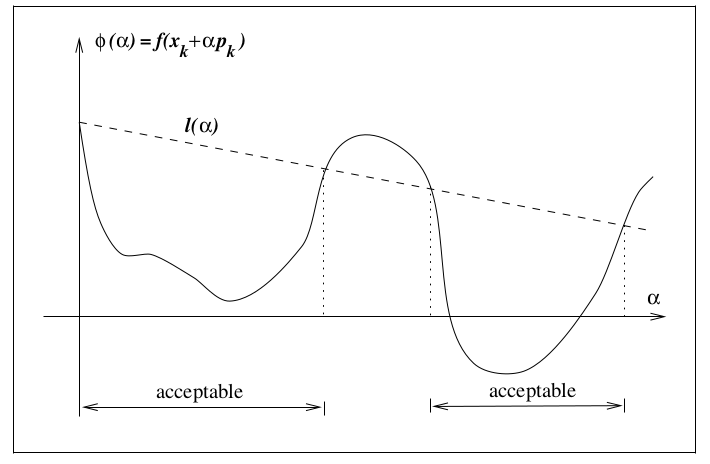
\includegraphics[height=3cm]{figures/armijo.png}
\end{minipage}
\begin{minipage}{0.48\textwidth}
\centering
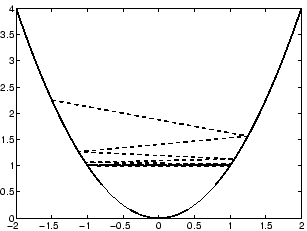
\includegraphics[height=3cm]{figures/armijo2.png}
\end{minipage}

\end{figure}

  \begin{equation*}
    l(\alpha) = f(x_k) + c_1 \alpha \nabla f_{k}^\intercal p_k, \; c_1 \in (0,1)
  \end{equation*}


\end{frame}

\begin{frame}
  \begin{equation*}
    \nabla f(x_k + \alpha p_k)^\intercal p_k \geq c_2 \nabla f_{k}^\intercal p_k, \; c_2 \in (c_1, 1)
  \end{equation*}

\begin{figure}
  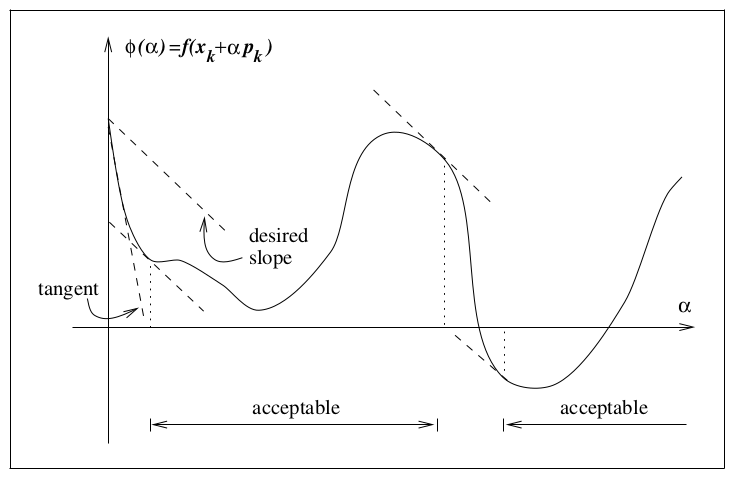
\includegraphics[height=5cm]{figures/curva.png}
\end{figure}

\end{frame}

\begin{frame}
  \frametitle{Strong Wolfe}
    \begin{equation*}
    f(x_k + \alpha p_k) \leq f(x_k) + c_1 \alpha \nabla f_{k}^\intercal p_k, \; c_1 \in (0,1)
  \end{equation*}

  \begin{equation*}
    \left| \nabla f(x_k + \alpha p_k)^\intercal p_k \right| \leq c_2 \left| \nabla f_{k}^\intercal p_k, \right| \; c_2 \in (c_1, 1)
  \end{equation*}

\begin{figure}
  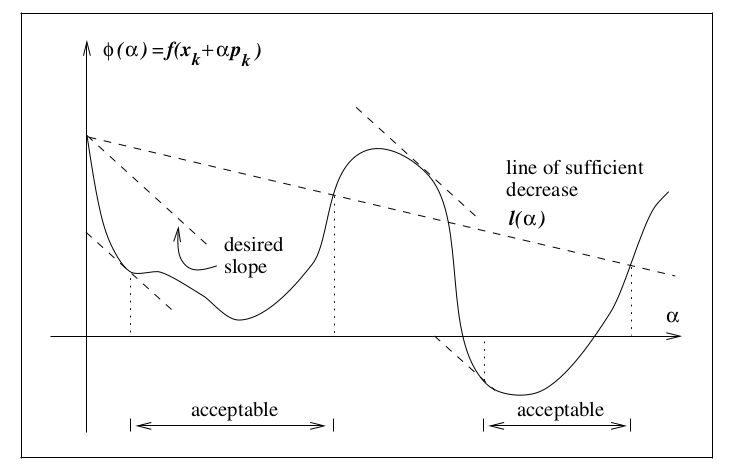
\includegraphics[height=5cm]{figures/strongWolfe.png}
\end{figure}

\end{frame}
